%%%%%%%%%%%%%%%%%%%%%%%%%%%%%%%%%%%%%%%%%%%%%%%%%%%%%%%%%%
%%
%%  LOD-L11.tex
%%  Lecture 11: Geometric Quantization by Paths
%%
%%%%%%%%%%%%%%%%%%%%%%%%%%%%%%%%%%%%%%%%%%%%%%%%%%%%%%%%%%

\chapter*{\S L11. Geometric Quantization by Paths}
\setcounter{footnote}{0}

%%%%%%%%%%%%%%%%%%%%%%%%%%%%%%%%%%%%%%%%%%%%%%%%%%%%%%%%%%
%%
%% MARK: Abstract
%%
%%%%%%%%%%%%%%%%%%%%%%%%%%%%%%%%%%%%%%%%%%%%%%%%%%%%%%%%%%
\begin{abstract}
  In this lecture,
  we shall see a new approach to prequantization that has been developed since the first edition of this book.
  Moving away from the traditional construction of principal bundles over the space of motions,
  we construct the \emph{Prequantum Groupoid} directly from the space of paths.
  This construction applies to any connected parasymplectic diffeological space,
  including singular quotients and infinite-dimensional spaces.
  It reveals that the quantum phase is not an external addition,
  but an intrinsic geometric property of the path space itself.
\end{abstract}

%%%%%%%%%%%%%%%%%%%%%%%%%%%%%%%%%%%%%%%%%%%%%%%%%%%%%%%%%%
%%
%% MARK: Introduction
%%
%%%%%%%%%%%%%%%%%%%%%%%%%%%%%%%%%%%%%%%%%%%%%%%%%%%%%%%%%%

Since the first publication of these lectures,
some notable progress has been made in the field of symplectic diffeology,
particularly regarding the problem of geometric quantization \cite{PIZ26a,PIZ26b}.

The traditional approach,
initiated by Kostant and Souriau,
relies on constructing a principal bundle (with structure group $\U(1)$ or $\RR$) over the symplectic manifold.
While powerful for smooth manifolds,
this approach encounters significant topological and structural obstructions when applied to the broader category of diffeological spaces.
Singular spaces,
such as orbifolds or leaf spaces of foliations,
often fail to admit such bundles in the standard sense,
or require heavy machinery like stacks or gerbes to be described.

However,
diffeology suggests a return to the source:
the space of paths.
Inspired by Feynman's path integral intuition,
but treated with rigorous geometry,
we propose that the fundamental object of quantization is not a bundle over the base space $X$,
but a quotient of the space of paths $\Paths(X)$.

This construction yields the \emph{Prequantum Groupoid}.
This object unifies the classical system and the quantum geometry into a single structure.
It naturally handles non-simply connected spaces,
irrational periods,
and singularities,
without leaving the framework of diffeology.

%%%%%%%%%%%%%%%%%%%%%%%%%%%%%%%%%%%%%%%%%%%%%%%%%%%%%%%%%%
%%
%% MARK: The Quantum Broth
%%
%%%%%%%%%%%%%%%%%%%%%%%%%%%%%%%%%%%%%%%%%%%%%%%%%%%%%%%%%%
\section{The Quantum Broth}

Let $(X,\omega)$ be a connected parasymplectic diffeological space.
That is,
$\omega$ is a closed $2$-form on $X$,
without further assumptions.

\begin{Article}{The Action Form.}{}
  We recall the existence of the chain-homotopy operator $\CHO$,
  introduced in earlier chapters.
  It maps $k$-forms on $X$ to $(k-1)$-forms on the space of paths $\Paths(X)$.
  The fundamental property of this operator is that for all $\alpha \in \DForms^k(X)$:
  $$%
    d[\CHO\alpha] + \CHO[d\alpha] = \1^*(\alpha) - \0^*(\alpha),
  $$%
  where $\0$ and $\1$ are the source and target maps from $\Paths(X)$ to $X$.

  Let us define the \emph{Action Form} on paths:
  $$%
    \Komega \in \DForms^1(\Paths(X)).
  $$%
  Explicitly,
  for a plot $P : U \to \Paths(X)$,
  the value of $\Komega$ is given by integrating $\omega$ along the variation of the paths:
  $$%
    (\Komega)(P)_r(\delta r) = \int_0^1 \omega \left( \Vector{t \\ r} \mapsto P(r)(t) \right)_{t \choose r} \Vector{1 \\ 0} \Vector{0 \\ \delta r} dt.
  $$%
  We call it the \emph{Action Form} because of its relationship with the classical action functional.
  In the case where $\omega = d\lambda$ is exact (e.g., cotangent bundles),
  the chain-homotopy formula gives:
  $$
    \Komega = \1^*(\lambda) - \0^*(\lambda) - dS,
  $$
  where $S(\gamma) = \int_\gamma \lambda = \CHO\lambda(\gamma)$ is the action functional.
  Thus,
  on the space of paths with fixed endpoints,
  $\Komega = -dS$.
  However,
  unlike the action functional $S$ which depends on the choice of a primitive $\lambda$,
  the Action Form $\Komega$ is always globally defined for any parasymplectic space $(X,\omega)$.

\end{Article}

\begin{Article}{The Primordial System.}{}
  We call the pair $(\Paths(X), \Komega)$ the \emph{Quantum Broth}.
  It contains all the information of the system:
  every possible history (path) and its associated symplectic potential.
  However,
  this space is immense and redundant.
  Geometric quantization,
  in this view,
  is the process of \emph{distilling} this broth.
  We want to identify paths that are physically indistinguishable from the perspective of the symplectic action.
\end{Article}

%%%%%%%%%%%%%%%%%%%%%%%%%%%%%%%%%%%%%%%%%%%%%%%%%%%%%%%%%%
%%
%% MARK: The Group of Periods
%%
%%%%%%%%%%%%%%%%%%%%%%%%%%%%%%%%%%%%%%%%%%%%%%%%%%%%%%%%%%
\section{The Group of Periods}

To define when two paths are equivalent,
we must understand the periodicity of the system.
The integration of $\Komega$ on loops is not always zero;
it detects the "holes" and the geometry of $X$.

\begin{Article}{The Total Group of Periods.}{}
  Let $\Loops(X)$ be the space of loops in $X$.
  Since $d\omega=0$,
  the restriction of $\Komega$ to $\Loops(X)$ is a closed $1$-form.
  Its periods generate a subgroup of $\RR$.
  However,
  if $X$ is not simply connected,
  we must also account for the non-commutativity of the fundamental group.

  We define the \emph{Total Group of Periods} $\Periods_\omega$ as the subgroup of $\RR$ generated by three sources:

  1. \emph{Spherical Periods:} Integrals of $\omega$ over contractible spheres (elements of $\pi_2(X)$),
  the loops in the connected component of the constant loop in $\Loops(X)$.

  2. \emph{Toric Periods:} Integrals of $\Komega$ over loops of $\Loops(X)$,
  within all the other connected components of the loop space.

  3. \emph{Surfacic Periods:} Integrals of $\omega$ over surfaces bounded by the commutators of the fundamental group $\pi_1(X)$,
  generated by the linking \emph{surfacic} cocycle between different connected components of the space of loops.

  We assume that $\Periods_\omega$ is a discrete subgroup of $\RR$ (i.e., $\Periods_\omega \neq \RR$).
  We define the \emph{Torus of Periods} as:
  $$%
    \Torus_\omega = \RR / \Periods_\omega.
  $$%
  This torus will play the role of the structure group (the phase) of our quantum system.
\end{Article}

%%%%%%%%%%%%%%%%%%%%%%%%%%%%%%%%%%%%%%%%%%%%%%%%%%%%%%%%%%
%%
%% MARK: The Prequantum Groupoid
%%
%%%%%%%%%%%%%%%%%%%%%%%%%%%%%%%%%%%%%%%%%%%%%%%%%%%%%%%%%%
\section{The Prequantum Groupoid}

We can now distill the Quantum Broth.
We define an equivalence relation on $\Paths(X)$ that identifies paths differing only by a "quantum period".

\begin{Article}{The Equivalence Relation.}{}
  Let $\gamma$ and $\gamma'$ be two paths in $X$.
  We say that $\gamma \sim_\omega \gamma'$ if:

  1. They share the same endpoints: $\Ends(\gamma) = \Ends(\gamma')$.

  2. The symplectic area enclosed by their concatenation is a period:
  $$%
    \int_{\gamma'}^\gamma \Komega \in \Periods_\omega.
  $$%
  Here,
  the integral is taken over any homotopy connecting $\gamma'$ to $\gamma$ in the space of paths with fixed endpoints.
  It can also be interpreted literally: the action needs to \emph{transmute} from path $\gamma$ to path $\gamma'$.

  Thanks to the definition of $\Periods_\omega$,
  this condition is well-defined even if the paths are not homotopic (the difference would be a surfacic period).
\end{Article}

\begin{Article}{The Groupoid Structure.}{}
  The quotient space $\cY = \Paths(X) / \sim_\omega$ forms the space of morphisms of a groupoid $\Torus_\omega$.

  \uline{Definition.} {\itshape The \emph{Prequantum Groupoid} $\Torus_\omega$ is defined by:
  \begin{itemize}
    \item Objects: $\Obj(\Torus_\omega) = X$.
    \item Morphisms: $\Mor(\Torus_\omega) = \cY$.
    \item Composition: Induced by the concatenation of paths,
    $$%
    [\gamma]_\omega \cdot [\gamma']_\omega = [\gamma \vee \gamma']_\omega.
    $$%
  \end{itemize}
  }

  This groupoid captures the geometry of the system perfectly.
  The classical space $X$ is embedded in it as the skeleton of identity morphisms (constant paths).
  The "quantum" nature lies in the non-identity morphisms.
\end{Article}

\begin{Article}{Isotropy and Phase.}{}
  A crucial feature of this construction is the structure of the isotropy group at a point $x \in X$:
  $$%
    \TT_{\omega, x} = \{ [\ell]_\omega \mid \ell \in \Loops(X,x) \}.
  $$%
  \uline{Theorem.} {\itshape For any point $x$,
  the isotropy group $\TT_{\omega, x}$ is isomorphic to the Torus of Periods $\Torus_\omega$.}

  This result is significant.
  It shows that the quantum phase ($\U(1)$ or $\Torus_\omega$) is not an external structure imposed on the system.
  It emerges intrinsically from the geometry of the paths and the periods of $\omega$.
\end{Article}

\begin{Article}{The Prequantum Form.}{}
  The Action Form $\Komega$ on the path space descends to the groupoid.

  \uline{Theorem.} {\itshape There exists a unique $1$-form $\blambda$ on $\cY$ such that:
  $$%
    \Class_\omega^*(\blambda) = \Komega.
  $$%
  This form is left-right invariant and its curvature satisfies:
  $$%
    d\blambda = \Trg^*(\omega) - \Src^*(\omega).
  $$%
  }
  The pair $(\Torus_\omega, \blambda)$ constitutes the \emph{Quantum System},
  which is composed of the Skeleton (the classical underlying system represented by the units) and the Quantum Fog (the non-identity morphisms, or \emph{transmutation channels}).

  Note that the primordial Quantum Broth $(\Paths(X),\Komega)$ is not forgotten;
  it remains as a legitimate diffeological structure on top of the Quantum System.
\end{Article}

%%%%%%%%%%%%%%%%%%%%%%%%%%%%%%%%%%%%%%%%%%%%%%%%%%%%%%%%%%
%%
%% MARK: Symmetries and the Moment Map
%%
%%%%%%%%%%%%%%%%%%%%%%%%%%%%%%%%%%%%%%%%%%%%%%%%%%%%%%%%%%
\section{Symmetries and the Moment Map}

One of the most elegant results of this construction concerns the symmetries.
In the classical bundle approach,
lifting symmetries often requires central extensions (like the Heisenberg group or the metaplectic correction).
Here,
the situation is simpler.

\begin{Article}{The Automorphism Group.}{}
  Let $\Aut(\Torus_\omega, \blambda)$ be the group of automorphisms of the groupoid that preserve the prequantum form.

  \uline{Theorem.} {\itshape The group of quantum symmetries is isomorphic to the group of classical symmetries:
  $$%
    \Aut(\Torus_\omega, \blambda) \simeq \Diff(X, \omega).
  $$%
  }
  This means that every classical symmetry lifts faithfully to the prequantum groupoid.
  The "quantum anomalies" or central extensions only appear when we try to represent this groupoid on a specific Hilbert space of sections (polarization),
  or when we arbitrarily fix a base point $x \in X$,
  but not at the global geometric level.
\end{Article}

\begin{Article}{The Quantum Moment Map.}{}
  In Lecture 10,
  we introduced the "paths moment map" $\Psi$.
  We can now reveal its true nature.
  Since $\Psi$ is constant on the equivalence classes of $\sim_\omega$ (up to the holonomy),
  it descends to the groupoid.

  The map $\Psi$ defined in the previous lecture is precisely the intrinsic moment map of the Prequantum Groupoid $\Torus_\omega$.
  The "holonomy" $\Gamma$ discussed previously is simply the image of the isotropy group $\Torus_\omega$ under this moment map.
\end{Article}

%%%%%%%%%%%%%%%%%%%%%%%%%%%%%%%%%%%%%%%%%%%%%%%%%%%%%%%%%%
%%
%% MARK: Examples
%%
%%%%%%%%%%%%%%%%%%%%%%%%%%%%%%%%%%%%%%%%%%%%%%%%%%%%%%%%%%
\section{Examples}

\begin{Article}{The Irrational Sphere Product.}{}
  Consider the product of two spheres $X = \Sph^2 \times \Sph^2$,
  equipped with the symplectic form $\omega = s_1 \Surf_1 + s_2 \Surf_2$,
  where $\Surf_i$ is the standard area form on the $i$-th sphere.
  The group of periods is generated by the integrals of $\omega$ over the two factors:
  $$
    \Periods_\omega = s_1 \ZZ + s_2 \ZZ.
  $$
  If the ratio $s_1/s_2$ is irrational,
  this group is dense in $\RR$.
  Standard geometric quantization fails here because the integrality condition (that periods must lie in $2\pi\ZZ$) cannot be satisfied.

  In our framework,
  the Torus of Periods $\Torus_\omega = \RR / (s_1 \ZZ + s_2 \ZZ)$ is an irrational torus (a quasifold).
  The prequantum groupoid $\Torus_\omega$ exists and is well-defined.
  Its isotropy is this irrational torus.
  This shows that diffeology allows us to quantize systems that are classically considered "unquantizable".
\end{Article}

\begin{Article}{The Aharonov-Bohm Effect.}{}
  Consider the punctured plane $X = \RR^2 - \{0\}$ with $\omega=0$.
  The groupoid is flat,
  but the geometry of $X$ creates a non-trivial holonomy for the moment map.
  The prequantum groupoid captures the magnetic flux through the hole via the geometry of the paths,
  even though the local curvature is zero.
  The "multi-valued" nature of the coupling is resolved into a single-valued function on the groupoid.
\end{Article}

\begin{Article}{Conclusion.}{}
  The Prequantum Groupoid offers a robust geometric foundation for quantization.
  It replaces the "bundle over a manifold" with a "quotient of paths".
  In doing so,
  it reconciles the symplectic geometry of Souriau with the path integral intuition of Feynman,
  all within the rigorous setting of diffeology.
\end{Article}

\vfill
\centerline{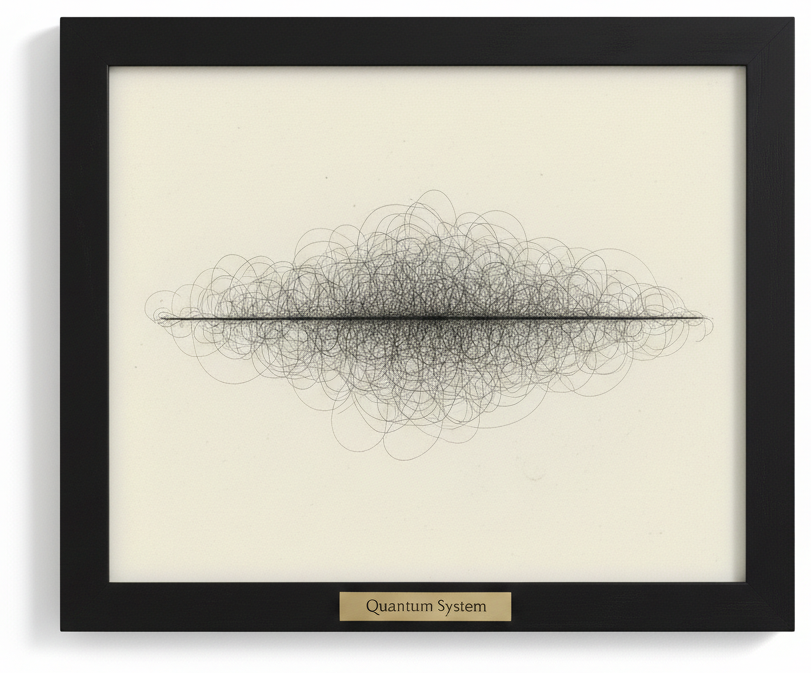
\includegraphics[width=.75\textwidth]{Figures/QuantumSystem.png}}
\vfill

%\begin{figure}[htbp]\n
%  \centering\n
%  % Replace 'QuantumSystemFrame.jpg' with your actual filename\n
%  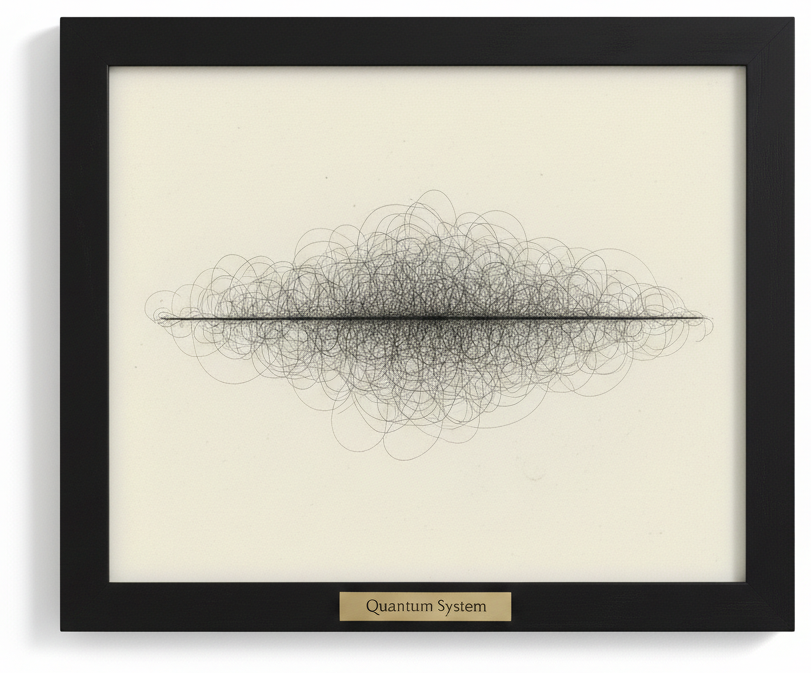
\includegraphics[width=0.85\textwidth]{Figures/QuantumSystem.png}\n
%  \caption[The Quantum System]{\n
%    \textbf{The Quantum System.}\n
%    An artistic visualization of the Prequantum Groupoid.\n
%    The horizontal line represents the \emph{Classical Skeleton} $X$ (the space of units).\n
%    The chaotic filaments represent the \emph{Quantum Broth} of paths $\Paths(X)$ emanating from and returning to the classical states.\n
%    The groupoid structure is the geometric distillation of this noise into a precise algebraic object.\n
%  }\n
%  \label{fig:QuantumSystem}\n
%\end{figure}\n
